% Todas as linhas precedidas pelo simbolo '%' são comentários
% e não afetam em nada o seu texto final.

% IGNORE. Pacotes necessários e acessórios para o documento
\documentclass[12pt]{exam}
 \usepackage{graphicx}
\usepackage{amsthm}
\usepackage{libertine}
\usepackage[utf8]{inputenc}
\usepackage[margin=1in]{geometry}
\usepackage{amsmath,amssymb}
\usepackage{multicol}
\usepackage[brazil]{babel}
\usepackage[shortlabels]{enumitem}
% ---

% Informações que podem ser configuradas
% ---
\newcommand{\class}{Matemática básica} % Nome da disciplina
\newcommand{\term}{2023}              % Perído Letivo
\newcommand{\examnum}{Monitoria de cálculo L1A}      % Número/Nome do exercício.
\newcommand{\examdate}{13/12/2023}        % insere a data no documento
\newcommand{\timelimit}{}               % IGNORE
\newcommand{\euler}{e}
% ---



\begin{document} % declaração de que o documento começa aqui.
\pagestyle{plain}
\thispagestyle{empty}
% ... formatação do cabeçalho
\noindent
\begin{tabular*}{\textwidth}{l @{\extracolsep{\fill}} r @{\extracolsep{6pt}} l}
 \textbf{\class} & \textbf{Monitores:} & \textit{Eduardo Guimarães}\\             % Insira o seu nome dentro dos {}'.
\textbf{\term} &&\\
\textbf{\examnum} &&\\
\textbf{\examdate} &&\\
\end{tabular*}\\
\rule[2ex]{\textwidth}{2pt}
% ---


\section{Derivada Geral de $ f(x)^{g(x)} $}


\begin{questions}
\question Calcule as seguintes derivadas.
    \begin{multicols}{2}
        \begin{enumerate}[(a)]
            \item
            $\displaystyle f(x)^{g(x)} \text{, } f(x) > 0 $
            \item 
            $\displaystyle g(x) = \left( 3 + \cos(x) \right)^x $
            \item 
            $\displaystyle y = x^x\sin(x) $
            \item 
            $\displaystyle y = x^\alpha $, onde $\alpha \in \mathbb{R}$
        \end{enumerate}
    \end{multicols}
\end{questions}


\section{Derivação Implicíta}

\begin{questions}
    \question Encontre a derivada de y em relação a x.
    \begin{multicols}{2}
        \begin{enumerate}[(a)]
            \item 
            $y^2 + xy - 1 = 0$
            \item 
            $y^3 + y = x$
            \item 
            $ y = \arctan(x)$
            \item 
            $ y = x^{x^3}$
        \end{enumerate}
    \end{multicols}
    
\end{questions}

\section{Pssição, Velocidade e Aceleração. Taxas Relacionadas}

\begin{questions}

\question A equação do movimento de uma partícula que se desloca ao longo o eixo x é $x = e^{-t}\sin{t}$, $t \geq 0$.
    \begin{multicols}{2}
        \begin{enumerate}[(a)]
            \item 
            Determine a vecolidade e aceleração no instante t.
            \item 
             Calcule $\displaystyle \lim_{t \to +\infty}  e^{-t}\sin{t} $
            \item 
            Esboce o gráfico da função.
            \item 
            Interprete tal movimento.
        \end{enumerate}
    \end{multicols}

\question Enche-se um reservatório, cuja forma é um cone cirular reto, de água a uma taxa de 0,1$m^3/s$. O vértice está a 15m do topo e o raio do topo mede 10m. Com que velocidade o nível h da água está subindo no instante em que h = 5m.

\begin{figure}[h]
    \centering
    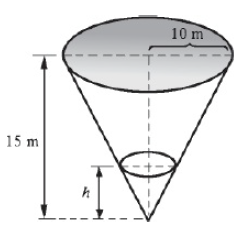
\includegraphics[width=3.5cm]{Screenshot_2.png}
    \caption{Caption}
    \label{fig:enter-label}
\end{figure}


\end{questions}
\end{document}
